\documentclass{standalone}
\usepackage{tikz}
\usetikzlibrary{patterns, positioning}


\begin{document}
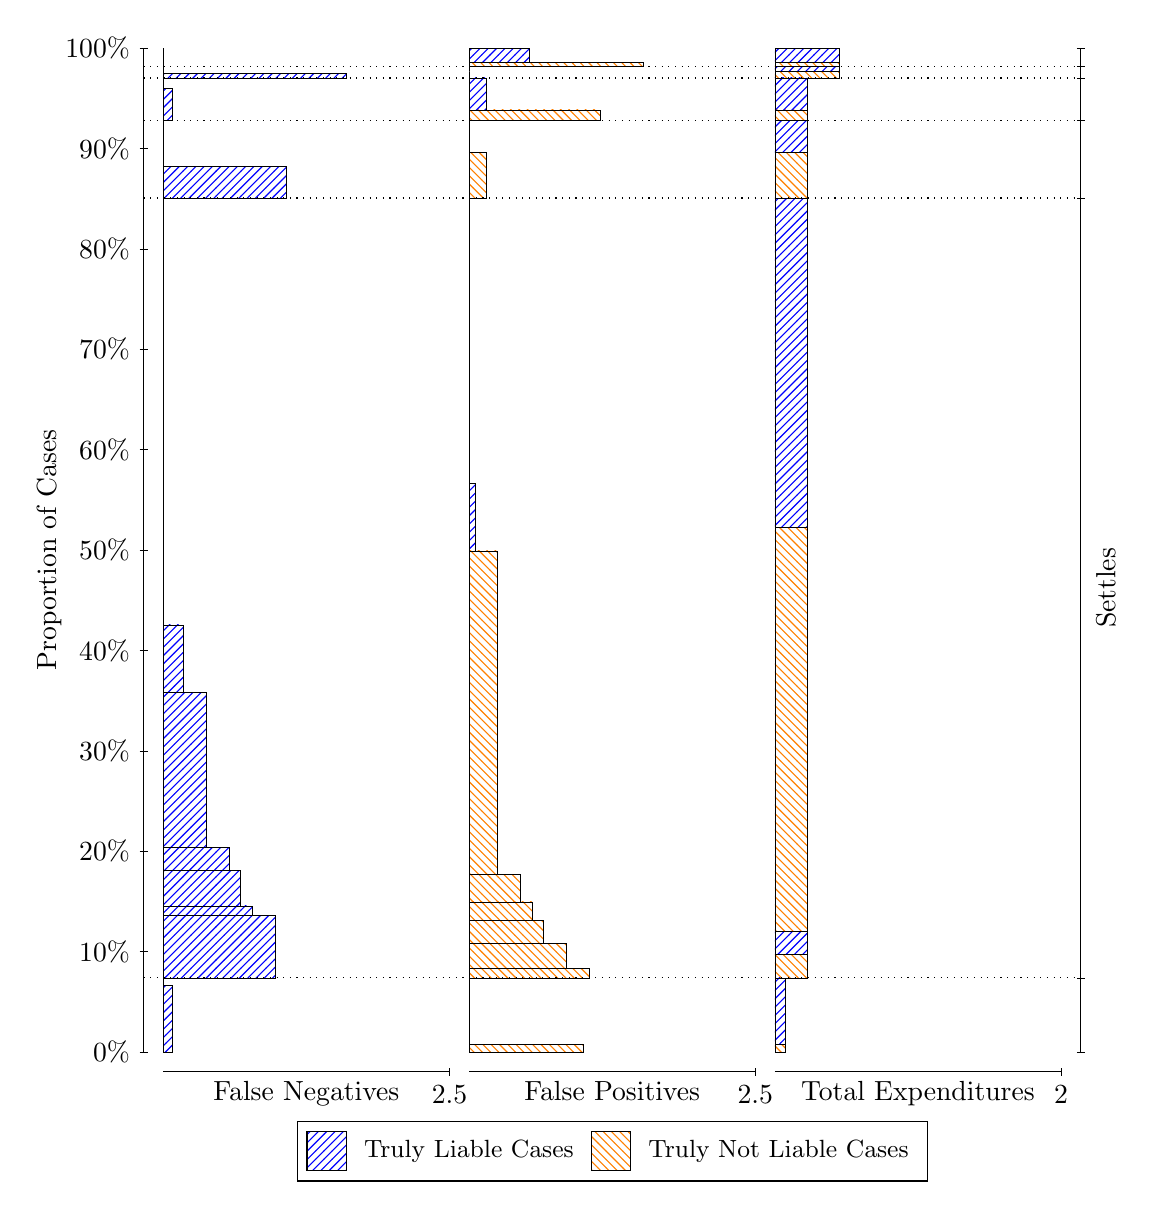
\begin{tikzpicture}
\draw[black, very thin] (1.5,1.75) -- (1.5,14.5);
\node[rotate=90, text=black, anchor=center] at (0.3, 8.125) {Proportion of Cases};
\draw[black, very thin] (1.45,1.75) -- (1.55,1.75);
\node[text=black, anchor=east] at (1.45, 1.75) {0\%};
\draw[black, very thin] (1.45,3.025) -- (1.55,3.025);
\node[text=black, anchor=east] at (1.45, 3.025) {10\%};
\draw[black, very thin] (1.45,4.3) -- (1.55,4.3);
\node[text=black, anchor=east] at (1.45, 4.3) {20\%};
\draw[black, very thin] (1.45,5.575) -- (1.55,5.575);
\node[text=black, anchor=east] at (1.45, 5.575) {30\%};
\draw[black, very thin] (1.45,6.85) -- (1.55,6.85);
\node[text=black, anchor=east] at (1.45, 6.85) {40\%};
\draw[black, very thin] (1.45,8.125) -- (1.55,8.125);
\node[text=black, anchor=east] at (1.45, 8.125) {50\%};
\draw[black, very thin] (1.45,9.4) -- (1.55,9.4);
\node[text=black, anchor=east] at (1.45, 9.4) {60\%};
\draw[black, very thin] (1.45,10.675) -- (1.55,10.675);
\node[text=black, anchor=east] at (1.45, 10.675) {70\%};
\draw[black, very thin] (1.45,11.95) -- (1.55,11.95);
\node[text=black, anchor=east] at (1.45, 11.95) {80\%};
\draw[black, very thin] (1.45,13.225) -- (1.55,13.225);
\node[text=black, anchor=east] at (1.45, 13.225) {90\%};
\draw[black, very thin] (1.45,14.5) -- (1.55,14.5);
\node[text=black, anchor=east] at (1.45, 14.5) {100\%};

\draw[black, very thin] (13.4,1.75) -- (13.4,14.5);
\draw[black, very thin] (13.35,1.75) -- (13.45,1.75);
\node[anchor=west] at (13.35, 1.75) {};
\draw[black, very thin] (13.35,2.6921) -- (13.45,2.6921);
\node[anchor=west] at (13.35, 2.6921) {};
\draw[black, very thin] (13.35,12.595) -- (13.45,12.595);
\node[anchor=west] at (13.35, 12.595) {};
\draw[black, very thin] (13.35,13.577) -- (13.45,13.577);
\node[anchor=west] at (13.35, 13.577) {};
\draw[black, very thin] (13.35,14.12) -- (13.45,14.12);
\node[anchor=west] at (13.35, 14.12) {};
\draw[black, very thin] (13.35,14.262) -- (13.45,14.262);
\node[anchor=west] at (13.35, 14.262) {};
\draw[black, very thin] (13.35,14.5) -- (13.45,14.5);
\node[anchor=west] at (13.35, 14.5) {};

\draw[black, very thin, pattern color=blue, pattern=north east lines] (1.75,1.75) rectangle (1.859,2.593);
\draw[black, very thin, pattern color=orange, pattern=north west lines] (1.75,2.593) rectangle (1.75,2.6921);
\draw[black, very thin, pattern color=blue, pattern=north east lines] (1.75,2.6921) rectangle (3.167,3.4813);
\draw[black, very thin, pattern color=blue, pattern=north east lines] (1.75,3.4813) rectangle (2.8763,3.6045);
\draw[black, very thin, pattern color=blue, pattern=north east lines] (1.75,3.6045) rectangle (2.731,4.0533);
\draw[black, very thin, pattern color=blue, pattern=north east lines] (1.75,4.0533) rectangle (2.5857,4.3509);
\draw[black, very thin, pattern color=blue, pattern=north east lines] (1.75,4.3509) rectangle (2.295,6.3147);
\draw[black, very thin, pattern color=blue, pattern=north east lines] (1.75,6.3147) rectangle (2.0043,7.1742);
\draw[black, very thin, pattern color=orange, pattern=north west lines] (1.75,7.1742) rectangle (1.75,12.595);
\draw[black, very thin, pattern color=blue, pattern=north east lines] (1.75,12.595) rectangle (3.3123,13);
\draw[black, very thin, pattern color=orange, pattern=north west lines] (1.75,13) rectangle (1.75,13.577);
\draw[black, very thin, pattern color=blue, pattern=north east lines] (1.75,13.577) rectangle (1.859,13.984);
\draw[black, very thin, pattern color=orange, pattern=north west lines] (1.75,13.984) rectangle (1.75,14.12);
\draw[black, very thin, pattern color=blue, pattern=north east lines] (1.75,14.12) rectangle (4.0753,14.179);
\draw[black, very thin, pattern color=orange, pattern=north west lines] (1.75,14.179) rectangle (1.75,14.262);
\draw[black, very thin, pattern color=orange, pattern=north west lines] (1.75,14.262) rectangle (1.75,14.321);
\draw[black, very thin, pattern color=blue, pattern=north east lines] (1.75,14.321) rectangle (1.75,14.5);
\draw[black, very thin, pattern color=orange, pattern=north west lines] (5.6333,1.75) rectangle (7.0867,1.8491);
\draw[black, very thin, pattern color=blue, pattern=north east lines] (5.6333,1.8491) rectangle (5.6333,2.6921);
\draw[black, very thin, pattern color=orange, pattern=north west lines] (5.6333,2.6921) rectangle (7.1593,2.8124);
\draw[black, very thin, pattern color=orange, pattern=north west lines] (5.6333,2.8124) rectangle (6.8687,3.1277);
\draw[black, very thin, pattern color=orange, pattern=north west lines] (5.6333,3.1277) rectangle (6.578,3.4205);
\draw[black, very thin, pattern color=orange, pattern=north west lines] (5.6333,3.4205) rectangle (6.4327,3.6556);
\draw[black, very thin, pattern color=orange, pattern=north west lines] (5.6333,3.6556) rectangle (6.2873,4.007);
\draw[black, very thin, pattern color=orange, pattern=north west lines] (5.6333,4.007) rectangle (5.9967,8.1133);
\draw[black, very thin, pattern color=blue, pattern=north east lines] (5.6333,8.1133) rectangle (5.706,8.9728);
\draw[black, very thin, pattern color=blue, pattern=north east lines] (5.6333,8.9728) rectangle (5.6333,12.595);
\draw[black, very thin, pattern color=orange, pattern=north west lines] (5.6333,12.595) rectangle (5.8513,13.172);
\draw[black, very thin, pattern color=blue, pattern=north east lines] (5.6333,13.172) rectangle (5.6333,13.577);
\draw[black, very thin, pattern color=orange, pattern=north west lines] (5.6333,13.577) rectangle (7.3047,13.714);
\draw[black, very thin, pattern color=blue, pattern=north east lines] (5.6333,13.714) rectangle (5.8513,14.12);
\draw[black, very thin, pattern color=orange, pattern=north west lines] (5.6333,14.12) rectangle (5.6333,14.203);
\draw[black, very thin, pattern color=blue, pattern=north east lines] (5.6333,14.203) rectangle (5.6333,14.262);
\draw[black, very thin, pattern color=orange, pattern=north west lines] (5.6333,14.262) rectangle (7.8497,14.321);
\draw[black, very thin, pattern color=blue, pattern=north east lines] (5.6333,14.321) rectangle (6.3963,14.5);
\draw[black, very thin, pattern color=orange, pattern=north west lines] (9.5167,1.75) rectangle (9.6529,1.8491);
\draw[black, very thin, pattern color=blue, pattern=north east lines] (9.5167,1.8491) rectangle (9.6529,2.6921);
\draw[black, very thin, pattern color=orange, pattern=north west lines] (9.5167,2.6921) rectangle (9.9254,2.9849);
\draw[black, very thin, pattern color=blue, pattern=north east lines] (9.5167,2.9849) rectangle (9.9254,3.2825);
\draw[black, very thin, pattern color=orange, pattern=north west lines] (9.5167,3.2825) rectangle (9.9254,8.4108);
\draw[black, very thin, pattern color=blue, pattern=north east lines] (9.5167,8.4108) rectangle (9.9254,12.595);
\draw[black, very thin, pattern color=orange, pattern=north west lines] (9.5167,12.595) rectangle (9.9254,13.172);
\draw[black, very thin, pattern color=blue, pattern=north east lines] (9.5167,13.172) rectangle (9.9254,13.577);
\draw[black, very thin, pattern color=orange, pattern=north west lines] (9.5167,13.577) rectangle (9.9254,13.714);
\draw[black, very thin, pattern color=blue, pattern=north east lines] (9.5167,13.714) rectangle (9.9254,14.12);
\draw[black, very thin, pattern color=orange, pattern=north west lines] (9.5167,14.12) rectangle (10.334,14.203);
\draw[black, very thin, pattern color=blue, pattern=north east lines] (9.5167,14.203) rectangle (10.334,14.262);
\draw[black, very thin, pattern color=orange, pattern=north west lines] (9.5167,14.262) rectangle (10.334,14.321);
\draw[black, very thin, pattern color=blue, pattern=north east lines] (9.5167,14.321) rectangle (10.334,14.5);
\draw[black, dotted] (1.5,2.6921) -- (13.4,2.6921);
\draw[black, dotted] (1.5,12.595) -- (13.4,12.595);
\draw[black, dotted] (1.5,13.577) -- (13.4,13.577);
\draw[black, dotted] (1.5,14.12) -- (13.4,14.12);
\draw[black, dotted] (1.5,14.262) -- (13.4,14.262);
\draw[black, very thin] (1.75,1.5) -- (5.3833,1.5);
\node[text=black, anchor=north] at (3.5667, 1.5) {False Negatives};
\draw[black, very thin] (5.3833,1.45) -- (5.3833,1.55);
\node[text=black, anchor=north] at (5.3833, 1.45) {2.5};

\draw[black, very thin] (5.6333,1.5) -- (9.2667,1.5);
\node[text=black, anchor=north] at (7.45, 1.5) {False Positives};
\draw[black, very thin] (9.2667,1.45) -- (9.2667,1.55);
\node[text=black, anchor=north] at (9.2667, 1.45) {2.5};

\draw[black, very thin] (9.5167,1.5) -- (13.15,1.5);
\node[text=black, anchor=north] at (11.333, 1.5) {Total Expenditures};
\draw[black, very thin] (13.15,1.45) -- (13.15,1.55);
\node[text=black, anchor=north] at (13.15, 1.45) {2};


\node[text=black, centered, rotate=90] at (13.72, 7.6437) {Settles};





\draw (7.449999999999999,1.5) node[draw=none] (baseCoordinate) {};
\begin{scope}[align=center]
        \matrix[scale=0.5, draw=black, below=0.5cm of baseCoordinate, nodes={draw}, column sep=0.1cm]{
            \node[rectangle, draw, minimum width=0.5cm, minimum height=0.5cm, pattern color=blue, pattern=north east lines] {}; &
            \node[draw=none, font=\small, text=black] (B) {Truly Liable Cases}; &
            \node[rectangle, draw, minimum width=0.5cm, minimum height=0.5cm, pattern color=orange, pattern=north west lines] {}; &
            \node[draw=none, font=\small, text=black] (B) {Truly Not Liable Cases}; \\
            };
\end{scope}

\end{tikzpicture}
\end{document}